\documentclass{standalone}
\usepackage{tikz}
\usetikzlibrary{shapes}

\tikzstyle{data}=[rectangle split,rectangle split parts=2,draw,text centered]
\newcommand{\data}{data \nodepart{second} \phantom{null}}

\begin{document}
	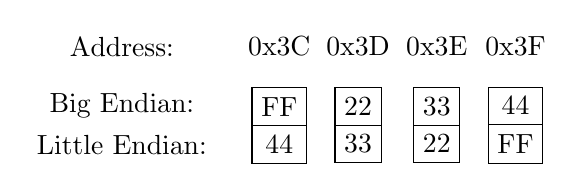
\begin{tikzpicture}
		\node[] (loc1) at (0,0) {0x3C};
		\node[right of=loc1] (loc2) {0x3D};
		\node[right of=loc2] (loc3)  {0x3E};
		\node[right of=loc3] (loc4) {0x3F};

		\node[] (address) at (-2,0){Address:};
		\node[data] (1) at (0,-1) {FF \nodepart{second} 44};
		\node[data] (2) at (1,-1) {22 \nodepart{second} 33};
		\node[data] (3) at (2,-1) {33 \nodepart{second} 22};
		\node[data] (4) at (3,-1) {44 \nodepart{second} FF};
		
		\node[] (be) at (-2,-0.75) {Big Endian:};
		\node[] (le) at (-2,-1.25) {Little Endian:};
	\end{tikzpicture}
\end{document}
